\documentclass[border=10pt]{standalone}

\usepackage{tikz}
\usepackage{tikzsymbols}
\usetikzlibrary{calc,patterns,shapes.geometric}

\def\centerarc[#1](#2)(#3:#4:#5){\draw[#1] ($(#2)+({#5*cos(#3)},{#5*sin(#3)})$) arc (#3:#4:#5);}

\begin{document}
	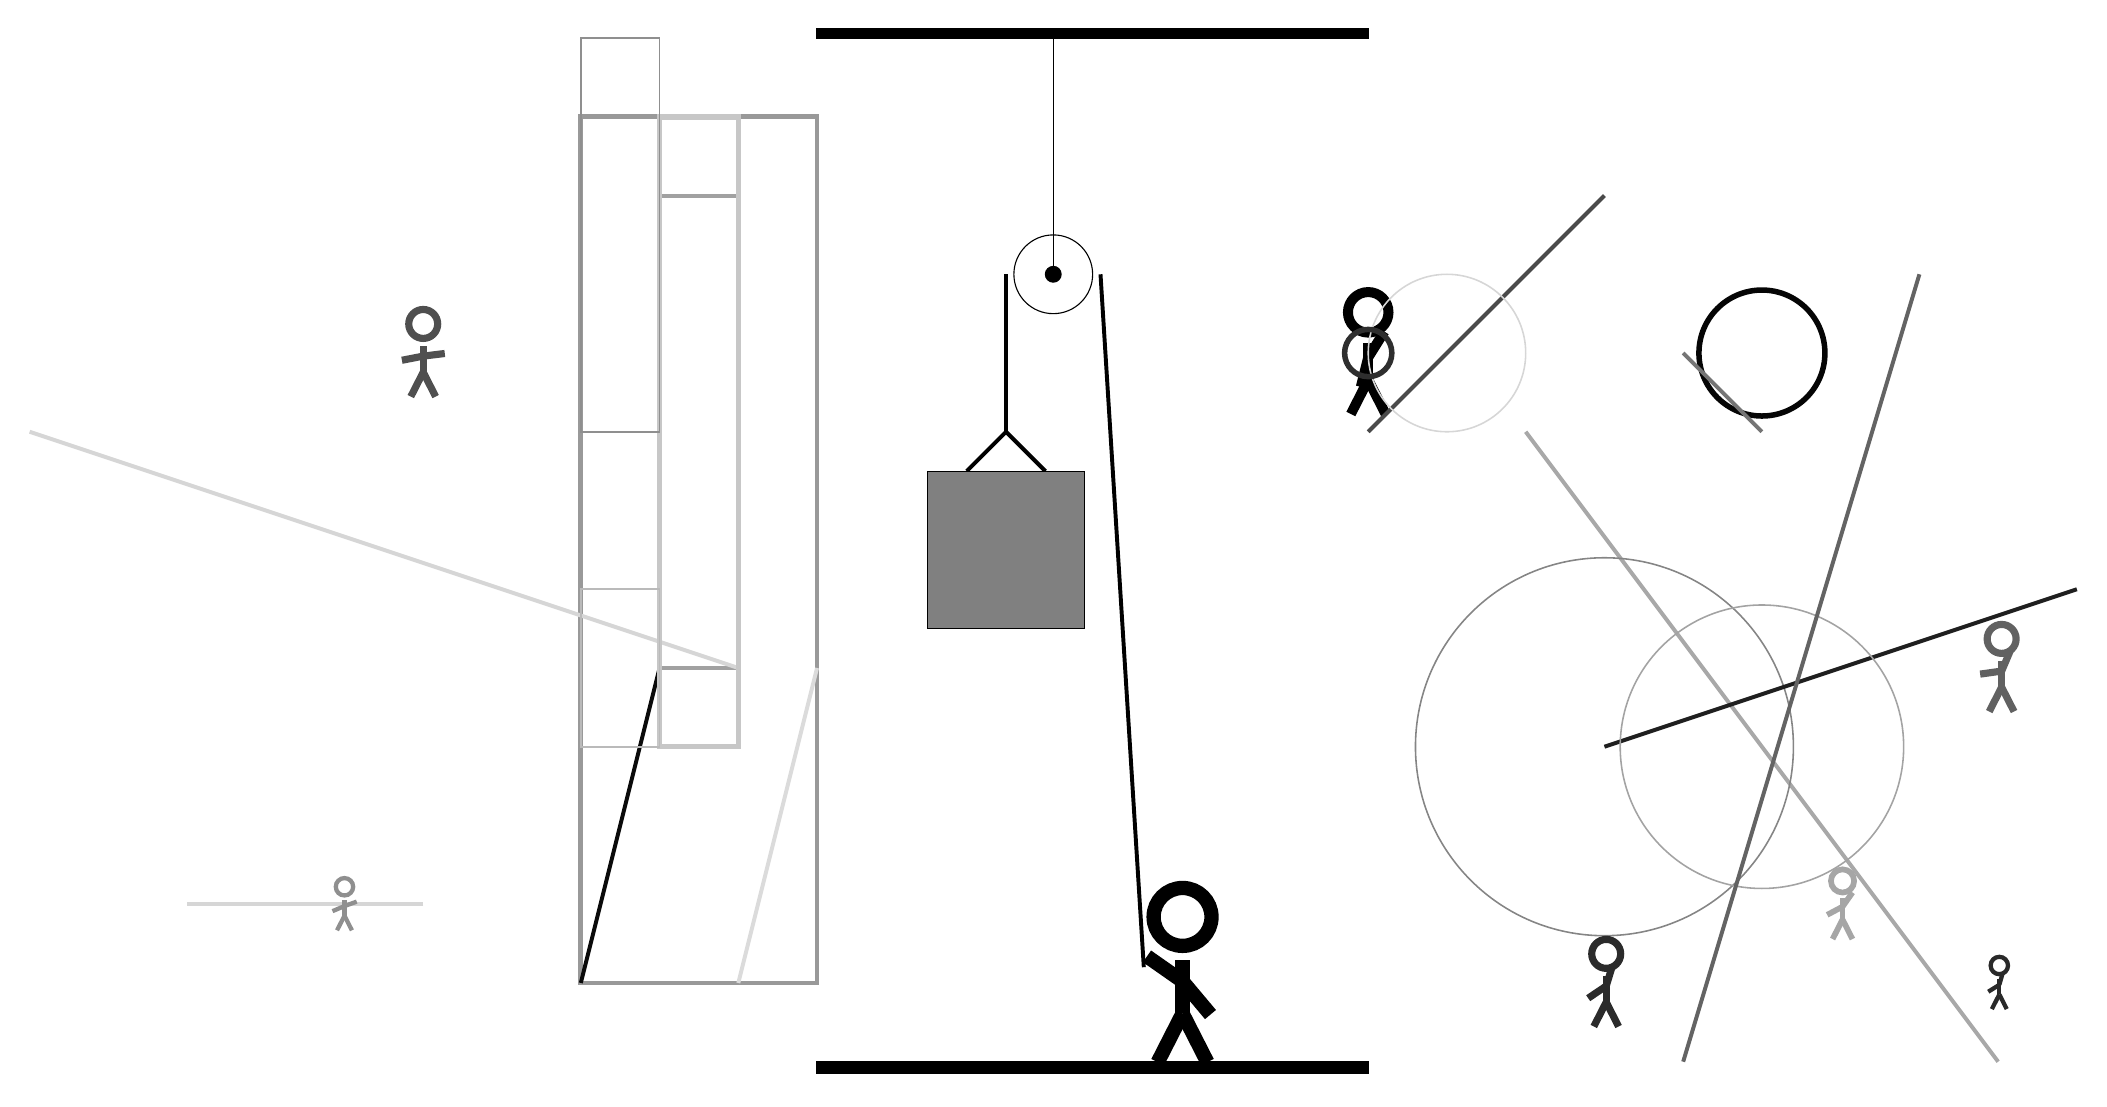
\begin{tikzpicture}
		%%%%% START %%%%%
		
		\draw[fill=black] (-2, 10) rectangle (5, 10.125);
		
		\draw [line width=0.7mm, color=black!98](10, 6) circle (0.8);
		
		\draw[line width=0.5mm, color=black!37] (-4, 2) rectangle (-3, 8);
		\draw[line width=0.6mm, color=black!40] (-2, 9) rectangle (-5, -2);
		\draw[line width=0.5mm, color=black!16](-7, -1) -- (-10, -1);
		\draw[line width=0.5mm, color=black!14](-2, 2) -- (-3, -2);
		
		\draw[line width=0.5mm, color=black!16](-3, 2) -- (-12, 5);
		\draw[line width=0.5mm, color=black!34](7, 5) -- (13, -3);
		
		\draw[line width=0.5mm, color=black!96](-5, -2) -- (-4, 2);
		\node[line width=0.4mm, color=black!35] at (11, -1) {\Strichmaxerl[4][28][55]};
		\draw[line width=0.7mm, color=black!22] (-3, 9) rectangle (-4, 1);
		\draw [line width=0.2mm, color=black!48](8, 1) circle (2.4);
		\draw[line width=0.5mm, color=black!88](8, 1) -- (14, 3);
		\draw [line width=0.2mm, color=black!36](10, 1) circle (1.8);
		
		\draw[line width=0.5mm, color=black!54](10, 5) -- (9, 6);
		\node[line width=0.7mm, color=black!62] at (13, 2) {\Strichmaxerl[5][8][67]};
		\draw[line width=0.5mm, color=black!61](9, -3) -- (12, 7);
		
		\node[line width=0.3mm, color=black!44] at (-8, -1) {\Strichmaxerl[3][23][20]};
		\draw[line width=0.2mm, color=black!44] (-4, 5) rectangle (-5, 10);
		\draw[line width=0.2mm, color=black!27] (-4, 3) rectangle (-5, 1);
		\node[line width=0.4mm, color=black!83] at (8, -2) {\Strichmaxerl[5][34][73]};
		\node[line width=0.4mm, color=black!84] at (13, -2) {\Strichmaxerl[3][32][74]};
		
		\node[line width=0.2mm, color=black!100] at (5, 6) {\Strichmaxerl[7][76][58]};
		\draw[line width=0.5mm, color=black!71](5, 5) -- (8, 8);
		\draw [line width=0.2mm, color=black!16](6, 6) circle (1.0);
		\node[line width=0.3mm, color=black!69] at (-7, 6) {\Strichmaxerl[5][11][7]};
		
		\draw [line width=0.7mm, color=black!82](5, 6) circle (0.3);
		
		\draw (1, 7) circle (0.5);
		\draw[fill=black] (1, 7) circle (0.1);
		\draw (1, 10) -- (1, 7);
		
		\draw[line width=0.5mm] (-0.1, 4.5) -- (0.4, 5.0) -- (0.9, 4.5);
		\draw[fill=black!50] (-0.6, 4.5) rectangle (1.4, 2.5);
		
		\draw[line width=0.5mm] (0.4, 7) -- (0.4, 5.0);
		\centerarc[line width=0.5mm](1, 7)(0:180:0.6);
		\draw[line width=0.5mm](1.6, 7) -- (2.15, -1.8);
		
		\node at (2.6, -1.9) {\Strichmaxerl[10][-35][-50]};
		
		\draw[fill=black] (-2, -3) rectangle (5, -3.15);
		
		%%%%% END %%%%%
	\end{tikzpicture}
\end{document}